\chapter{Optimizing the synthesis of monodisperse colloidal spheres}
\label{ch:synthesis}

Since the introduction of emulsion polymerization in XXX [XXX citation], synthesis of colloidal spheres has progressed through
intuitive leaps guided by fundamental principles of chemistry
and physics.  Quite often, the importance of particular chemical
or physical conditions to the outcome can only be gauged once
synthesis is complete, and requires multiple orthogonal measurement
techniques. Examples include measurements of the size distribution
of their particles, their surface texture, and their porosity.
Here, we explore the role of stoichiometry, initiator choice and
agitation conditions on the synthesis of
monodisperse spheres of
\num{3}-methacryloxypropyltrimethoxysilane (TPM),
a model system with increasingly widespread applications
in soft-matter research [XXX anything else?].
We employ holographic particle characterization
in tandem with conventional particle characterization
techniques
to identify factors that 
influence size selection, polydispersity and surface texture.

Spheres made from  \num{3}-methacryloxypropyltrimethoxysilane (TPM) are a 
particularly useful system for colloidal studies. Their synthesis readily 
produces monodisperse spheres in a wide range of sizes through a process 
that is simpler than that for other common colloidal particles, such 
as polystyrene and silica. There is no specialized 
equipment or inert environment necessary. The particles can be made 
in a single step through an order of magnitude of sizes, from a few 
hundred nanometers to a few micrometers. However, there are many 
parameters in the synthesis that can affect the final particle that 
is produced. In this study we vary a selection of these conditions 
and use holographic video microscopy to observe how they affect the 
final product of the synthesis.

% Plopping this into the paper as we don't have a structure yet.
\section{Experimental Section}
\subsection{Materials.}
TPM OIL ( what and purchased from where). Ammonia. Initiators. 
Stir bars. Vials (microcentrifuge). Heat/shaker.
tubes. xCells xSight.

\subsection{Emulsification Polymerization.}

All of the spheres in this study were made through an emulsion 
polymerization process. Monomeric TPM, which is insoluble in water, 
is added to a basic environment (pH $>$ \num{9}) of ammonia in water. The 
monomers undergo hydrolysis in the water and become water soluble. 
In a basic environment, these hydrolyzed monomers form insoluble 
oligomers. As the suspension is stirred, the oligomers condense 
homogeneously into monodisperse droplets that grow as more oligomers 
form. After \num{2} hours, this process is completed and the droplets have 
reached their final size. Once the droplets are formed, a free radical 
initiator is used to polymerize the droplets and form solid spheres.

The droplet formation is done in a closed vial to prevent the 
evaporation of the ammonia and maintain the pH throughout the droplet 
formation process. This suggests that the particular container used for 
the synthesis may affect the final product, as the amount of air above 
the suspension will affect how much ammonia is left in the water and 
therefore the pH of the environment. To control this, we used identical 
\SI{12}{\milli\liter} vials to make \SI{5}{\milli\liter} of colloidal 
suspension in each synthesis.

First, we investigate the effect of varying the stir speed of the 
suspensions during droplet formation. In four identical vials with 
identical stir bars, we \SI{15}{\milli\liter} of 
\SI{29}{\percent} ammonia followed by \SI{200}{\micro\liter} of TPM 
monomer to \SI{5}{\milli\liter} of DI water. The four samples are then stirred 
using magnetic stir plates set at \num{500}, \num{700}, \num{900}, and \SI{1100}{\minute^{-1}} for \SI{2}{\hour}. % XXX Use rpm instead of min^{-1}?
At this point the droplets have stopped growing and they are polymerized 
by adding \num{2},\num{2}'-azobis(\num{2}-methylpropionitrile) (AIBN) and 
heating to \SI{80}{\celsius} for \SI{2}{\hour}. 
%XXX Add conclusions about stir speed- surprisingly, the faster stir speed led to larger droplets...)

The polymerization of the TPM droplets can be tracked by observing the 
refractive index of the particles over time. As the droplets polymerize, 
their refractive index increases until they are fully polymerized. To track 
this, we sampled the suspension above that was stirred at \SI{1100}{\min^{-1}}
% XXX Again, rpm vs mins^{-1}
after \si{5}, \si{10}, \si{15}, \si{20}, \si{40}, and \SI{60}{\min} of 
heating and measured the particles' refractive index. 
%XXX (Add conclusions about polymerization time- only takes maybe 15 min?)

Next, we observe the effect of using different free radical initiators 
to polymerize the particles. Two water-insoluble initiators, AIBN and
\num{1},\num{1}'-azobis(cyclohexanecarbonitrile) (ACHN), and two water-soluble 
initiators, potassium persulfate (KPS) and ammonium persulfate APS), were 
used. To do this, one suspension of emulsion droplets is made and then 
divided into four vials. Each vial was then polymerized at \SI{80}{\celsius} 
for \SI{12}{\hour} on a shaker at \SI{750}{\minute^{-1}} % XXX Again, rpm vs mins^{-1}
to prevent sedimentation. 
We repeated this process with four different emulsions for a total of 
\num{16} measurements to ensure that any observations were the result of the 
initiator and not of the particular protocol used to make the emulsion.

To make the four batches of droplets, we hold the volume of water constant 
and vary the amounts of TPM and ammonia. Batches A and B each had 
\SI{100}{\micro\liter} of TPM with \si{10} and \SI{20}{\micro\liter} of 
ammonia added, respectively. Batches C and D had \SI{150}{\micro\liter}, 
again with \si{10} and \SI{20}{\micro\liter} of ammonia, respectively. 
The polymerization for all of the particles was done in \SI{0.1}{\percent} 
SDS to avoid aggregation. 
% XXX (Add conclusions about initiator- does not seem to matter)

In making the \si{16} sets of particles to look at the effect of initiator on 
the particles, we can also make observations about the effects of varying 
the amount of TPM and the pH on the size of the resulting droplets. To hold 
the pH constant, we can compare sample A to C and sample B to D. This gives 
the fairly intuitive result that increasing the amount of TPM increases the 
size of the final droplet. Holding the amount of TPM constant and varying 
the pH, which means comparing A to B and C to D, shows that increasing the 
pH of the environment during droplet formation decreases the size of the 
final droplet. This is less intuitive but perhaps not surprising, as the pH 
affects the rate at which oligomers form and therefore the rate of droplet 
formation. This leads to more nucleation sites and therefore smaller droplets 
for the same volume of material. 

\subsection{Characterization}

\section{Results and discussion}
\subsection{Role of Initiator.}

\subsection{Role of Heat Bath.}

\subsection{Role of Stir rate.}


\begin{figure}
    \centering
    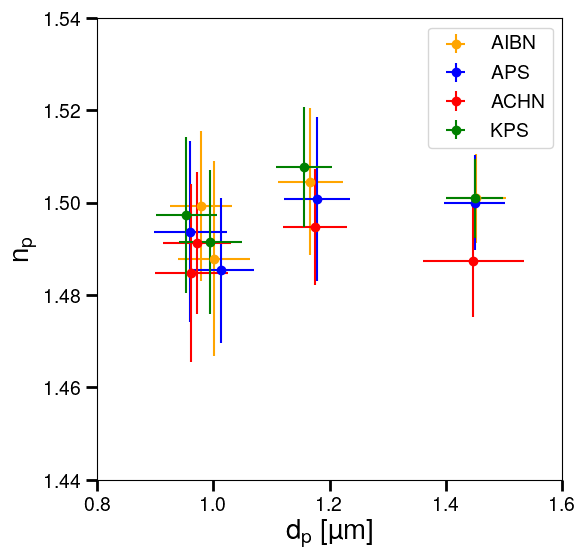
\includegraphics[width=0.75\columnwidth]{may_data_summary.png}
    \caption{The refractive index and diameter of 16 samples of 
    polymerized TPM.}
    \label{fig:initiator_data}
\end{figure}

\begin{figure}
    \centering
    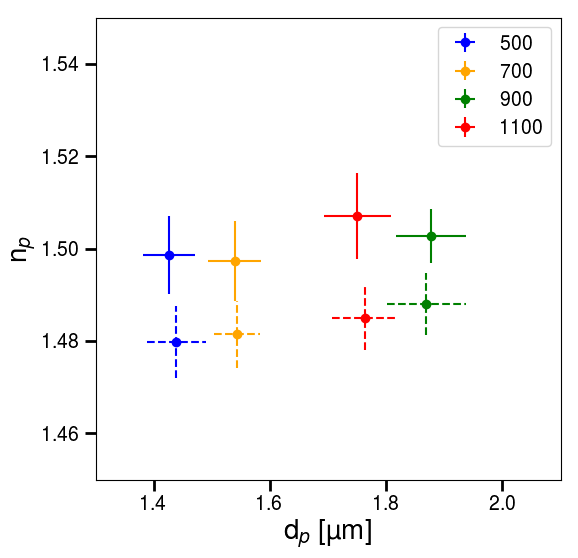
\includegraphics[width=0.75\columnwidth]{may_data_stirring_both}
    \caption{Caption}
    \label{fig:stir_rate}
\end{figure}


\section{Discussion}
